\section{Compensation-Conditioned Gait Scheduling}\label{sec:method}
\begin{figure}[t]
\centering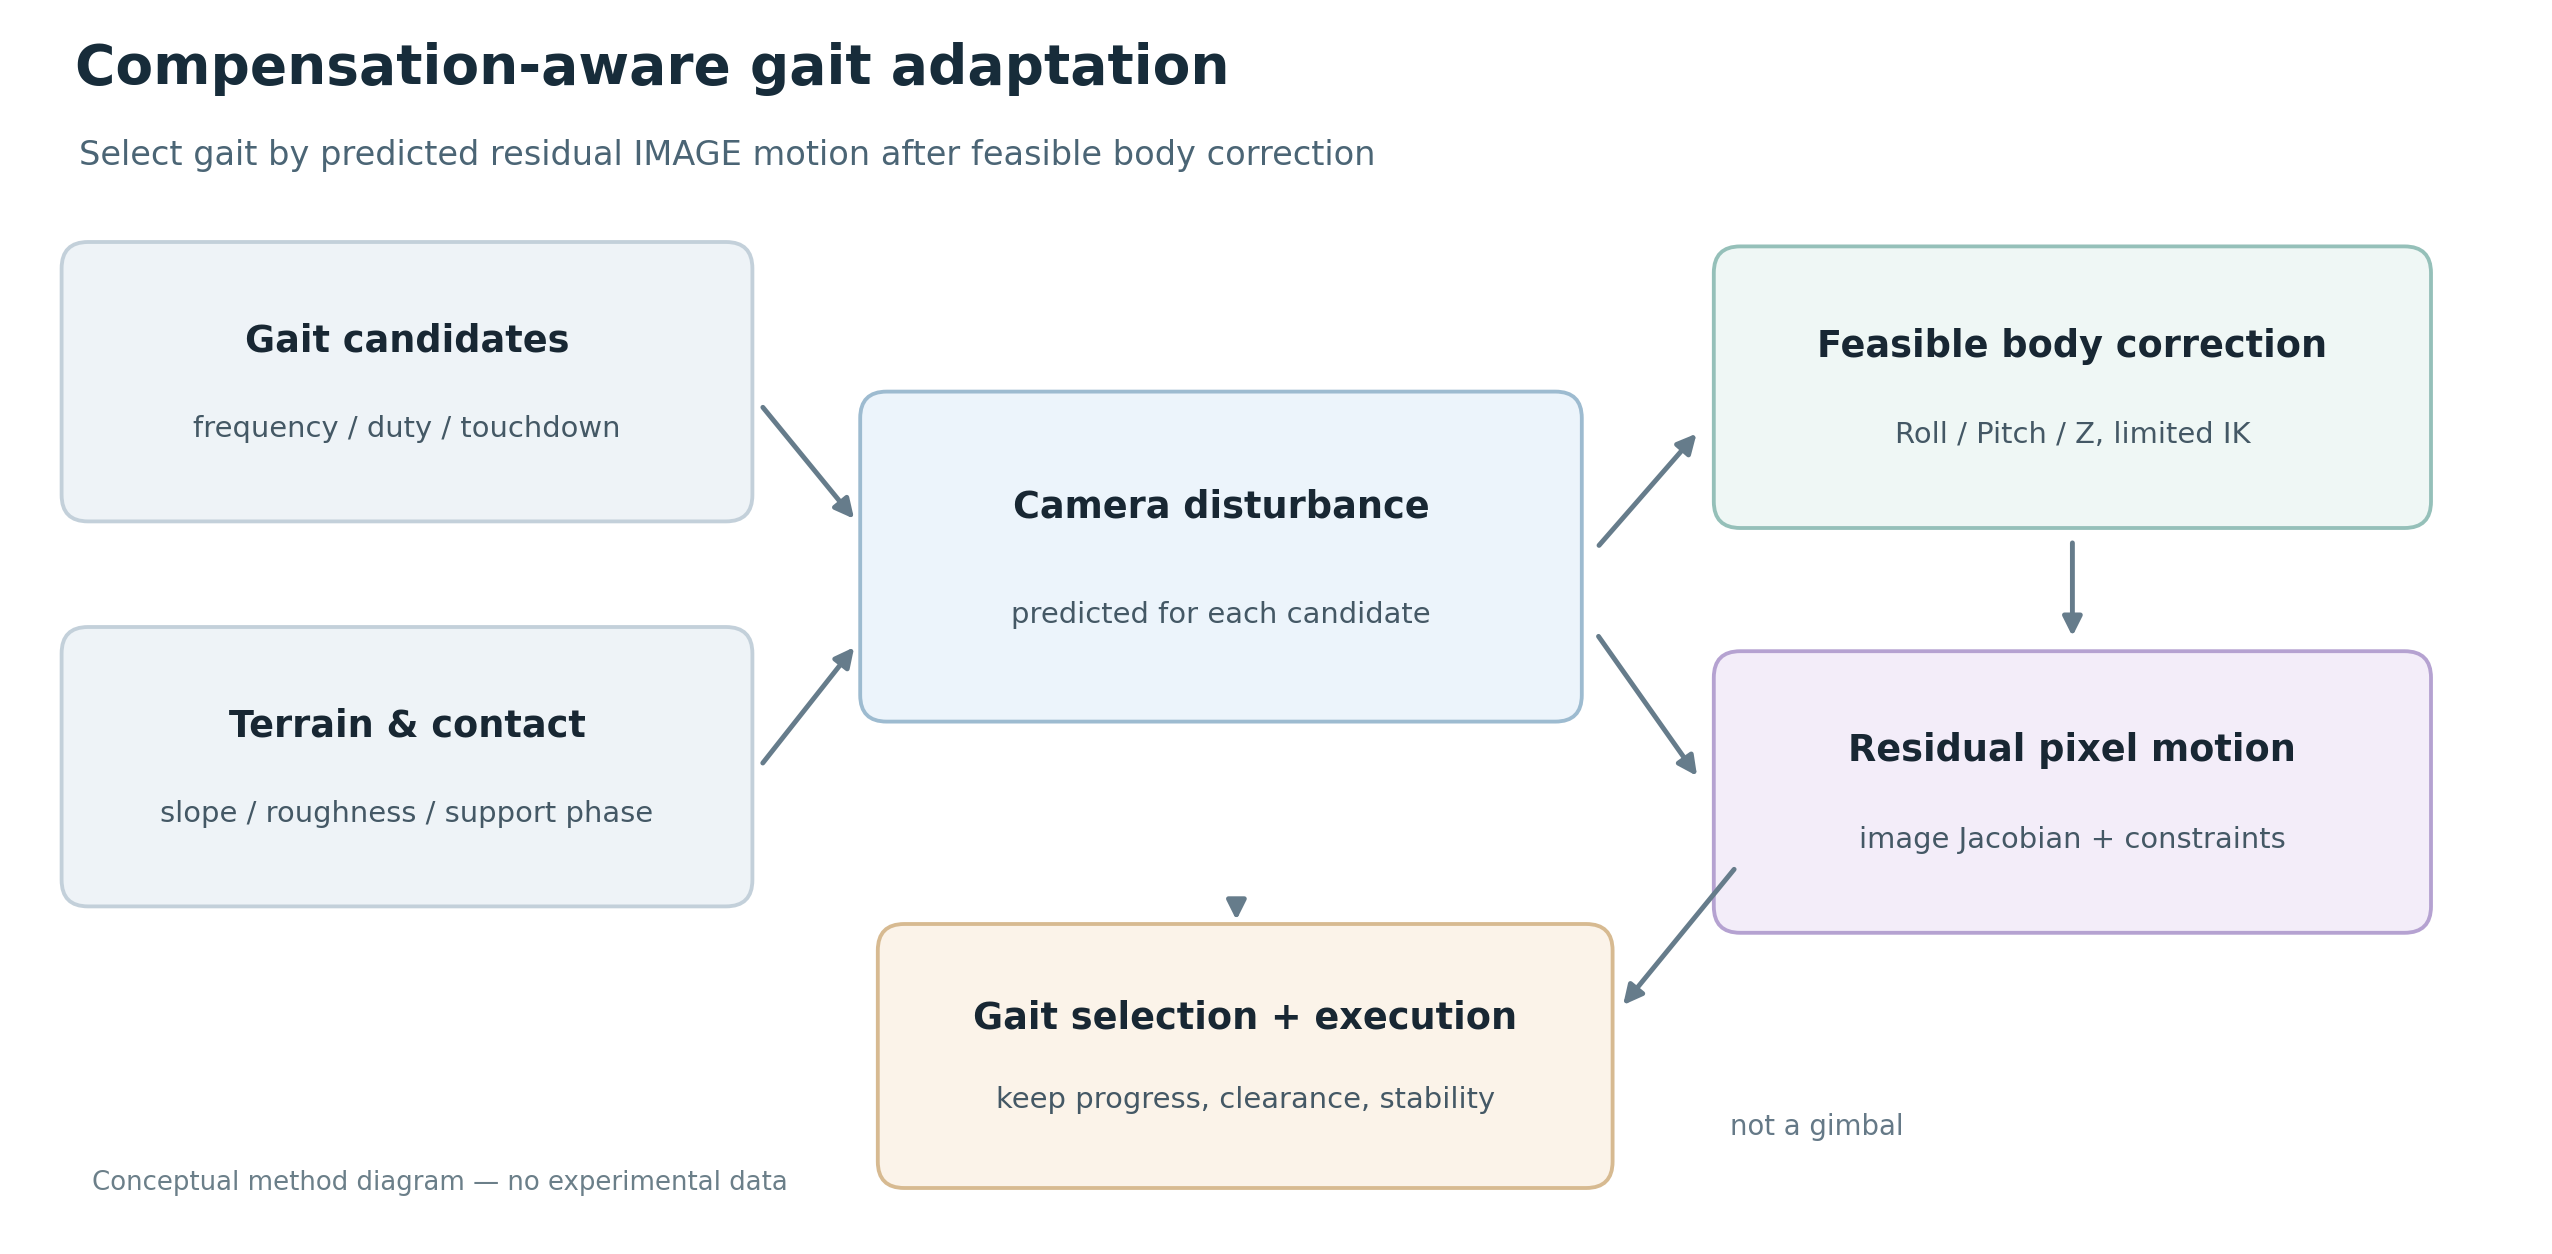
\includegraphics[width=\linewidth]{figures/Fig1_concept.png}
\caption{Research concept: a shared set of feasible gait candidates is evaluated using predicted gait-induced disturbance and the actual response of a fixed body stabilizer. The figure illustrates the proposed architecture and contains no experimental results.}\label{fig:concept}
\end{figure}

\subsection{Candidate generation and safe transitions}
We retain a phase-continuous alternating-tripod generator with gait parameters $\bm\theta=[f,\beta,\kappa]^\top$, where $f$ is cycle frequency, $\beta$ is the stance duty ratio, and $\kappa$ controls touchdown smoothness. The stride length is determined in conjunction with frequency and requested velocity rather than varied independently without regard to achieved speed. Swing height is set from required terrain clearance. A small neighborhood of candidate parameters is enumerated only at phase-safe transitions. The current gait and a verified fallback are always included.

The common locomotion layer checks joint position and velocity limits, stance-foot reachability, swing-foot clearance, and a support/contact safety condition for each candidate. Feasible correction is not inferred merely from available joint angle range. In particular, the nominally permissible body adjustment may still be impossible under foot-ground contact or actuator-response constraints. The online selector is never permitted to override the underlying safety controller.

\subsection{Gait-conditioned raw and closed-loop response prediction}
Let $\bm o_t$ collect only information available before choosing a gait: current joint and inertial states, gait phase, the preceding gait and time since the last change, available local terrain estimates, and predicted support/kinematic margins computed from the candidate trajectory. For the same candidate $\bm\theta$, we distinguish uncompensated disturbance $\bm d^{0,\bm\theta}$ from the residual $\bm r^{\pi,\bm\theta}$ when a \emph{fixed, physically executed} body-pose controller $\pi_c$ is enabled. Both are defined relative to the intended smooth camera motion from Section~\ref{sec:problem}; deliberate translation and navigation yaw are not treated as gait jitter.

A general candidate-conditioned formulation is
\begin{align}
\widehat{\bm d}^{0,\bm\theta}_{t:t+H}&=F_\psi(\bm o_t,\bm\theta,\widehat{\mathcal T}_t),\label{eq:predictor}\\
\widehat{\bm r}^{\pi,\bm\theta}_{t:t+H}&=G_\eta(\bm o_t,\bm\theta,\widehat{\bm d}^{0,\bm\theta}_{t:t+H};\pi_c).\label{eq:empiricalresponse}
\end{align}
Unlike an ideal inner minimization, $G_\eta$ must represent the \emph{achieved} response of $\pi_c$, including finite tracking bandwidth, support transitions and saturation. It need not assume that any kinematically reachable compensation command can be executed instantaneously.

The first executable surrogate predicts the short-window scalar image-motion costs $\widehat J^0(\bm o_t,\bm\theta)$ and $\widehat J^\pi(\bm o_t,\bm\theta)$ independently using small regularized regressors. These are trained on paired \emph{conditions} with the same gait parameterization, target speed, terrain realization and initial-state distribution, with the body stabilizer disabled/enabled, respectively. Such paired rollouts are not asserted to have identical subsequent robot trajectories. The effective reduction
\begin{equation}\label{eq:authorityproxy}
\widehat{\Delta J}_{\pi}(\bm\theta)=\widehat J^0(\bm\theta)-\widehat J^\pi(\bm\theta)
\end{equation}
is a measurable, controller-conditioned \emph{response proxy}, not a geometric wrench polytope or a proof of dynamic feasibility. It is allowed to be negative if compensation worsens camera stability. A separate regressor estimates the attained forward speed for candidate screening. Higher-dimensional camera-twist and multi-frequency models will be used only if their validation establishes additional value over this explicit baseline.

Crucially, the training observations must span \emph{different candidate gait settings}. Replaying the currently observed IMU trace under every candidate does not produce a counterfactual gait predictor. The training/test split is grouped by independent terrain realizations and seeds, and paired controller-on/off trials must remain in the same split. No future simulator contact state, privileged terrain ground truth or test-rollout achieved speed may be used as an online predictor input.

\subsection{Measured and support-dependent body response}
The same Roll, Pitch and vertical-body stabilization controller $\pi_c$ operates under every comparison method. Let $\bm b=[\delta z,\delta\phi,\delta\vartheta]^\top$ be its limited pose correction. For stance foot $i$ with an approximately fixed world contact point $\bm p_i^W$, the required leg-frame target is
\begin{equation}\label{eq:stanceanchor}
\bm p_i^B(\bm b)=\bm R_{WB}(\bm b)^\top(\bm p_i^W-\bm t_{WB}(\bm b)).
\end{equation}
The inverse kinematics must respect
\begin{equation}\label{eq:limits}
\bm q_{\min}\le\mathrm{IK}(\bm p_i^B)\le\bm q_{\max},\qquad
|\Delta\bm q_i|\le\dot{\bm q}_{\max}\Delta t.
\end{equation}
These are necessary but not sufficient conditions. Contact retention, slip, support margin and actual actuator response must also be checked or measured. Rather than inventing a frequency cut-off, we propose identification of the response between limited safe body-pose references and measured body/camera motion, with support conditions recorded. The empirical response model captures the effects of the existing controller in the tested domain; generality beyond observed speeds, surfaces and support states is not assumed.

\subsection{Residual image motion and supervisory decision}
Let $J^\pi(\bm\theta)$ measure unwanted image-plane motion \emph{after} the actual body compensator, obtained by projecting camera twist relative to the nominal motion through the image interaction matrix in Eq.~\eqref{eq:interaction} and integrating over camera frames. The projected per-frame RMS displacement is a reproducible kinematic proxy, not an actual photometric blur measurement. Independently recorded RGB trajectories provide the final visual metric by tracking static scene features and subtracting intentional navigation flow. Camera exposure, temporal synchronization and rolling-shutter effects must be controlled or reported.

The gait selection objective is
\begin{equation}\label{eq:outer_goal_new}
\begin{aligned}
\bm\theta_t^*=\arg\min_{\bm\theta\in\Theta_{\rm safe}}\quad
&\widehat J^\pi(\bm o_t,\bm\theta)+\lambda_s\|\bm\theta-\bm\theta_{t-1}\|_{\bm W}^2,\\
\mathrm{s.t.}\quad&\widehat v(\bm o_t,\bm\theta)\ge v_{\min}.
\end{aligned}
\end{equation}
Every candidate must first pass the same kinematic, contact and transition screens. The speed predictor is only a screening aid; measured achieved speed and traversal success remain decisive evidence. Parameter switching is restricted to safe phase boundaries and uses hysteresis to prevent chattering. If no candidate is admissible, the host controller retains its verified gait or stops safely.

\noindent\textbf{Algorithm 1:}\enspace At a gait update, (1) create a common, physically screened gait menu; (2) use the current state and locally available terrain estimates to predict short-window $\widehat J^0$, $\widehat J^\pi$ and achieved speed for each candidate; (3) reject candidates failing speed and support constraints; (4) select the feasible minimum of Eq.~\eqref{eq:outer_goal_new}; (5) enact parameter changes at a safe support transition while the unchanged fast body controller continues to run. The comparison selector differs \emph{only} by ranking candidates with $\widehat J^0$ instead of $\widehat J^\pi$.

\subsection{Identification, computational cost and scope}
We evaluate both predictors on held-out terrain realizations with absolute image-motion error, predicted ordering accuracy and top-one candidate regret; reporting averaged regression fit alone is insufficient. A dedicated mechanism study measures how frequently raw-motion and closed-loop-motion orderings differ across all candidate pairs, rather than showcasing a single favorable episode. An additional history-only residual-feedback selector determines whether counterfactual prediction improves adaptation beyond simple online tuning from previously executed gaits.

The current implementation uses a small standardized ridge model and finite menu search to keep computational overhead measurable. The number of evaluated candidates, mean and worst-case CPU time, rejected candidates and actual control-loop delay must be recorded on the target processor. This is a proposed method subject to evaluation, not a claimed real-time or performance result.
